\section{Thí nghiệm mở rộng}
Đánh giá khả năng nhận dạng chữ số viết tay của mô hình trên dữ liệu người Việt được nhóm thu thập qua ba thí nghiệm: (a) huấn luyện bằng MNIST; (b) bổ sung data augmentation; (c) kết hợp MNIST với một phần dữ liệu người Việt. Qua đó, đánh giá ảnh hưởng của lệch miền dữ liệu, hiệu quả cải thiện và xây dựng demo vẽ chữ số trực tiếp.
\subsection{Tập chữ số Việt}
\subsubsection{Thu thập và xử lý dữ liệu}
Mỗi người viết điền một phiếu in A4 gồm lưới $10\times10$ ô: mỗi hàng là một chữ số từ 0 đến 9, viết 10 lần theo cách tự nhiên, rồi ký xác nhận đồng ý cho sử dụng dữ liệu. Phiếu có bốn ô đen ở bốn góc làm dấu định vị. Nhóm thu được 30 phiếu từ 30 người viết (mã W01--W30), chụp bằng điện thoại.

Module \code{src/vn\_digits.py} chuyển ảnh phiếu sang định dạng MNIST qua các bước ở Hình~\ref{fig:vnpipe}. Bước cuối lặp lại đúng quy trình tạo MNIST (khung $20\times20$, căn khối tâm vào ảnh $28\times28$), nên khác biệt còn lại chủ yếu là khác biệt về nét viết chứ không phải do định dạng. Cả 3.000 ô đều có chữ (không ô trống); sau khi xem lại từng phiếu, nhóm loại 20 ô viết nhầm, gạch xoá hoặc bẩn (ghi trong \code{data/vn\_exclude.csv}), còn lại \textbf{2.980 ảnh}, mỗi lớp từ 294 đến 300 ảnh.

\begin{figure}[H]
\centering
\begin{tikzpicture}[
  box/.style={draw,rounded corners=2pt,fill=blue!6,align=center,font=\footnotesize,minimum height=1.05cm,text width=2.05cm},
  arr/.style={-{Stealth[length=2mm]},thick}, node distance=0.35cm]
  \node[box] (a) {Ảnh chụp\\phiếu};
  \node[box,right=of a] (b) {Tìm 4 ô đen,\\nắn phẳng\\phối cảnh};
  \node[box,right=of b] (c) {Cắt 100 ô\\theo lưới,\\bỏ lề ô};
  \node[box,right=of c] (d) {Tách nét khỏi\\nền, đảo màu\\(nền đen)};
  \node[box,right=of d] (e) {Cắt khung\\bao, thu về\\$20\times20$};
  \node[box,right=of e] (f) {Căn khối tâm\\vào $28\times28$};
  \foreach \u/\v in {a/b,b/c,c/d,d/e,e/f} \draw[arr] (\u) -- (\v);
\end{tikzpicture}
\caption{Quy trình chuyển ảnh chụp phiếu thành ảnh chữ số theo định dạng MNIST (\code{review\_sheet}, \code{process\_sheet}, \code{build\_dataset}).}
\label{fig:vnpipe}
\end{figure}

\begin{figure}[H]
  \centering
  \begin{minipage}[c]{0.27\linewidth}\centering
    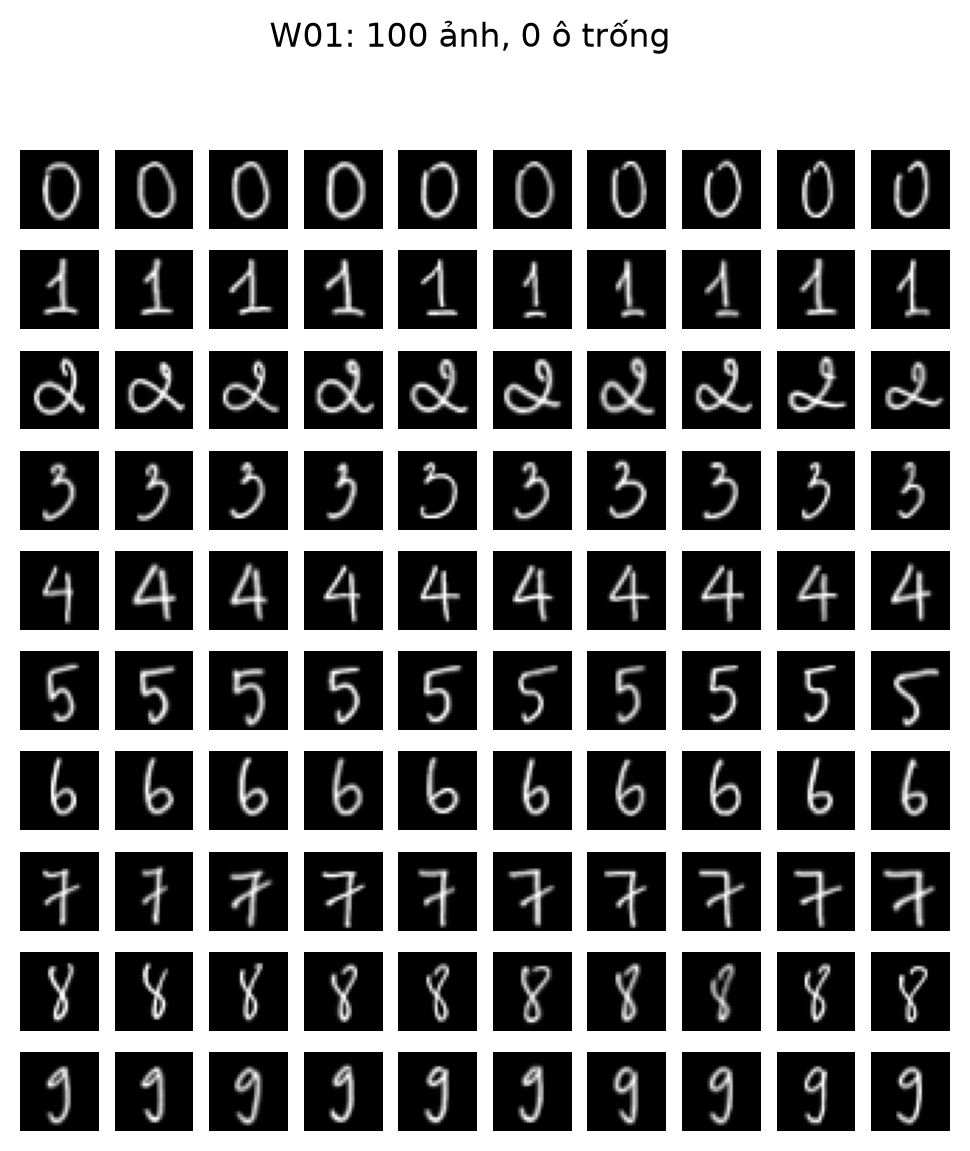
\includegraphics[width=\linewidth,trim=0 0 0 18,clip]{figures/vn_cells_W01.png}
    \subcaption{100 ô của phiếu W01}
  \end{minipage}\hfill
  \begin{minipage}[c]{0.7\linewidth}\centering
    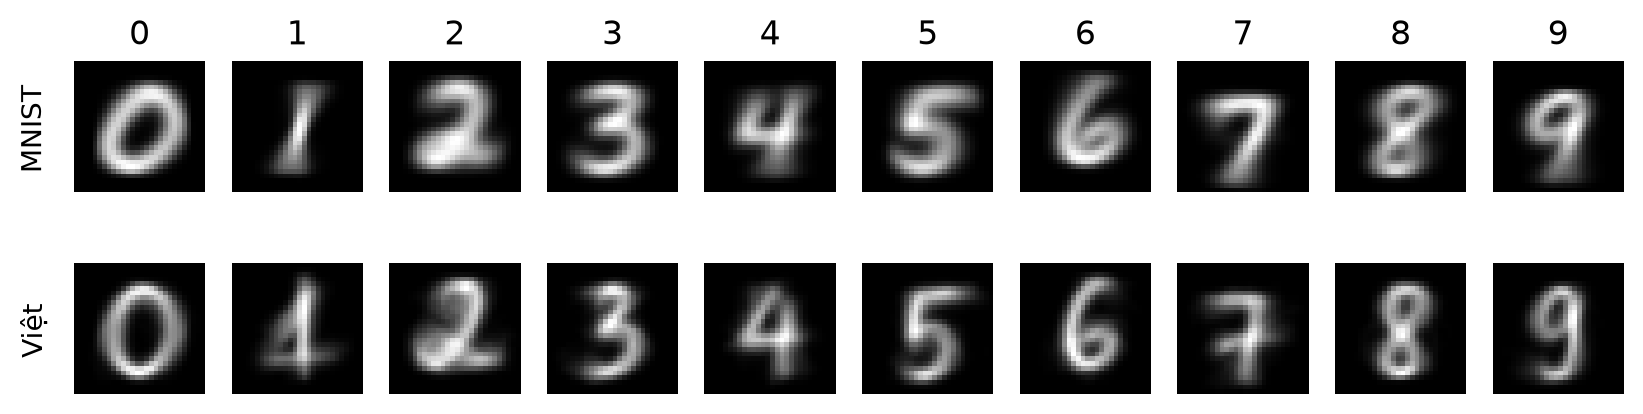
\includegraphics[width=\linewidth]{figures/vn_mean_images.png}
    \subcaption{Ảnh trung bình: MNIST (trên) và tập Việt (dưới)}
  \end{minipage}
  \caption{Tập chữ số người Việt sau khi xử lý. Ở ảnh trung bình, số 1 của người Việt có nét móc ở đầu và gạch chân, số 7 có gạch ngang ở giữa, và các chữ số nói chung đứng thẳng hơn MNIST.}
  \label{fig:vndata}
\end{figure}

\subsection{Datasheet}
Bảng~\ref{tab:datasheet} tóm tắt tập dữ liệu theo khung \emph{Datasheets for Datasets} %\cite{gebru2021}.

\begin{table}[H]
\centering
\caption{Datasheet của tập chữ số viết tay người Việt.}
\label{tab:datasheet}
\small
\begin{tabularx}{\linewidth}{@{}p{2.9cm}X@{}}
\toprule
Mục đích & Đo mức lệch miền giữa MNIST và chữ số người Việt; đánh giá augmentation và việc bổ sung ít dữ liệu đúng miền. \\
Thành phần & 2.980 ảnh xám $28\times28$, nhãn 0--9, mã người viết W01--W30; 294--300 ảnh/lớp, khoảng 100 ảnh/người. \\
Thu thập & Phiếu in A4 lưới $10\times10$ có 4 ô đen định vị; viết bằng bút bi và bút nước, chụp bằng điện thoại trong \todo{điều kiện ánh sáng}; thời gian \todo{tháng/năm}. \\
Tiền xử lý & Như Hình~\ref{fig:vnpipe}; 0 ô trống, loại thủ công 20 ô lỗi. Ảnh phiếu gốc được giữ riêng, không công bố. \\
Đồng ý \& riêng tư & Người viết ký xác nhận trên phiếu; dữ liệu công bố không chứa tên hay chữ ký, chỉ có mã người viết. \\
Hạn chế & 30 người viết nên chưa đại diện cho người Việt nói chung; mỗi người viết 10 lần liên tiếp nên các ảnh của cùng một người rất giống nhau. \\
Sử dụng & Chỉ dùng cho mục đích học tập trong môn học; không dùng để nhận diện người viết. \\
\bottomrule
\end{tabularx}
\end{table}

\subsubsection{Thiết kế thí nghiệm}
Bảng~\ref{tab:vnexp} mô tả ba thí nghiệm. Cả bốn bộ phân lớp dùng nguyên cấu hình đã chọn trên validation MNIST (Na\"{\i}ve Bayes $\alpha=0{,}001$; Logistic Regression $\eta=0{,}1$; MLP $(784,256,128,10)$; Random Forest 50 cây, độ sâu tối đa 15), \emph{không} chỉnh lại theo tập Việt.

\begin{table}[H]
\centering
\caption{Ba thí nghiệm về lệch miền.}
\label{tab:vnexp}
\small
\begin{tabularx}{\linewidth}{@{}lp{3.6cm}p{3.1cm}X@{}}
\toprule
& Huấn luyện trên & Kiểm tra trên & Câu hỏi \\
\midrule
(a) & MNIST & Người Việt & Lệch miền làm giảm bao nhiêu? Lớp nào, mô hình nào chịu ảnh hưởng nhất? \\
(b) & MNIST + augmentation & Người Việt & Dạy mô hình ``chịu'' xoay, dịch, nhiễu có giảm được lệch miền không? \\
(c) & MNIST + \emph{một phần} người Việt & \emph{Những người Việt còn lại} & Thêm một ít dữ liệu đúng miền giúp được bao nhiêu? \\
\bottomrule
\end{tabularx}
\end{table}

Tập Việt được chia \emph{theo người viết} (\code{writer\_split}, 30\% người viết làm tập kiểm tra): toàn bộ ảnh của một người chỉ nằm ở một phía. Nếu chia ngẫu nhiên theo ảnh, mô hình sẽ được kiểm tra trên chính nét chữ đã thấy khi huấn luyện và kết quả sẽ lạc quan giả tạo. Cả ba thí nghiệm được đánh giá trên \emph{cùng} nhóm người viết kiểm tra; việc chia được lặp với 3 hạt giống và báo cáo trung bình $\pm$ độ lệch chuẩn. Ở (b), mỗi ảnh MNIST được bổ sung một bản biến đổi ngẫu nhiên (xoay, dịch, nhiễu; \todo{tham số trong \code{augment\_dataset}}), tập huấn luyện tăng lên 108.000 ảnh. Ở (c), ảnh của những người viết thuộc phần huấn luyện được lặp lại 5 lần rồi ghép vào 54.000 ảnh MNIST, để vài nghìn ảnh Việt không bị lấn át.


\subsection{Tăng cường dữ liệu và thí nghiệm độ bền}

\subsubsection{Ý tưởng và cách cài đặt}

Tăng cường dữ liệu (\textit{Data Augmentation}) tạo thêm các biến đổi từ ảnh huấn luyện, giúp mô hình nhận dạng chữ số tốt
hơn khi hình ảnh bị thay đổi. Thí nghiệm độ bền (\textit{Robustness})
đánh giá khả năng duy trì độ chính xác khi ảnh đầu vào bị xoay,
dịch chuyển hoặc thêm nhiễu.

Hàm \texttt{augment\_dataset()} tạo thêm một bản biến đổi cho mỗi
ảnh huấn luyện (\texttt{copies=1}). Dữ liệu gốc và dữ liệu mới được
ghép lại, đồng thời giữ nguyên nhãn:
\[
X_{\mathrm{aug}}=[X_{\mathrm{tr}};X_{\mathrm{trans}}],
\qquad
y_{\mathrm{aug}}=[y_{\mathrm{tr}};y_{\mathrm{tr}}].
\]

Hàm \texttt{perturb()} tạo dữ liệu kiểm tra biến đổi theo ba phép:
xoay ảnh ở các góc $0^\circ,10^\circ,20^\circ,30^\circ,45^\circ$;
dịch ảnh chéo xuống-phải từ $0$ đến $4$ pixel; và thêm nhiễu
Gaussian với $\sigma\in\{0,0.1,0.2,0.3,0.5\}$.
Các mô hình được huấn luyện trên dữ liệu gốc và dữ liệu tăng cường,
sau đó đánh giá trên cùng tập kiểm tra đã biến đổi.

Độ chính xác được tính theo:
\[
\mathrm{Accuracy}=
\frac{1}{N}\sum_{i=1}^{N}
\mathbf{1}(\hat{y}_i=y_i),
\]
trong đó $N$ là số ảnh kiểm tra, $\hat{y}_i$ là nhãn dự đoán và
$y_i$ là nhãn thực tế.

\subsubsection{Kết quả thực nghiệm}

\begin{figure}[htbp]
    \centering

    % Bảng ở trên
    \begin{minipage}{\textwidth}
        \centering
        \captionof{table}{So sánh độ chính xác của các mô hình trên ảnh gốc,
ảnh xoay $30^\circ$ và ảnh dịch chuyển $3$ pixel (\%)}
        \label{tab:robustness}
        \small
        \begin{tabular}{lccc}
            \hline
            \textbf{Mô hình} &
            \textbf{Ảnh gốc} &
            \textbf{Xoay $30^\circ$} &
            \textbf{Dịch 3 pixel} \\
            \hline
            Logistic Regression       & 92.13 & 55.83 & 11.17 \\
            Logistic Regression + aug & 91.24 & 55.62 & 23.13 \\
            MLP                       & 98.09 & 78.44 & 20.19 \\
            MLP + aug                 & 98.58 & 86.88 & 77.91 \\
            Multinomial NB            & 83.64 & 44.75 & 16.72 \\
            Multinomial NB + aug      & 81.06 & 43.99 & 9.53 \\
            Random Forest             & 96.45 & 71.29 & 16.05 \\
            Random Forest + aug       & 96.18 & 77.49 & 37.39 \\
            \hline
        \end{tabular}
    \end{minipage}

    \vspace{0.5cm}

    % Hình ở dưới
    \begin{minipage}{\textwidth}
        \centering
        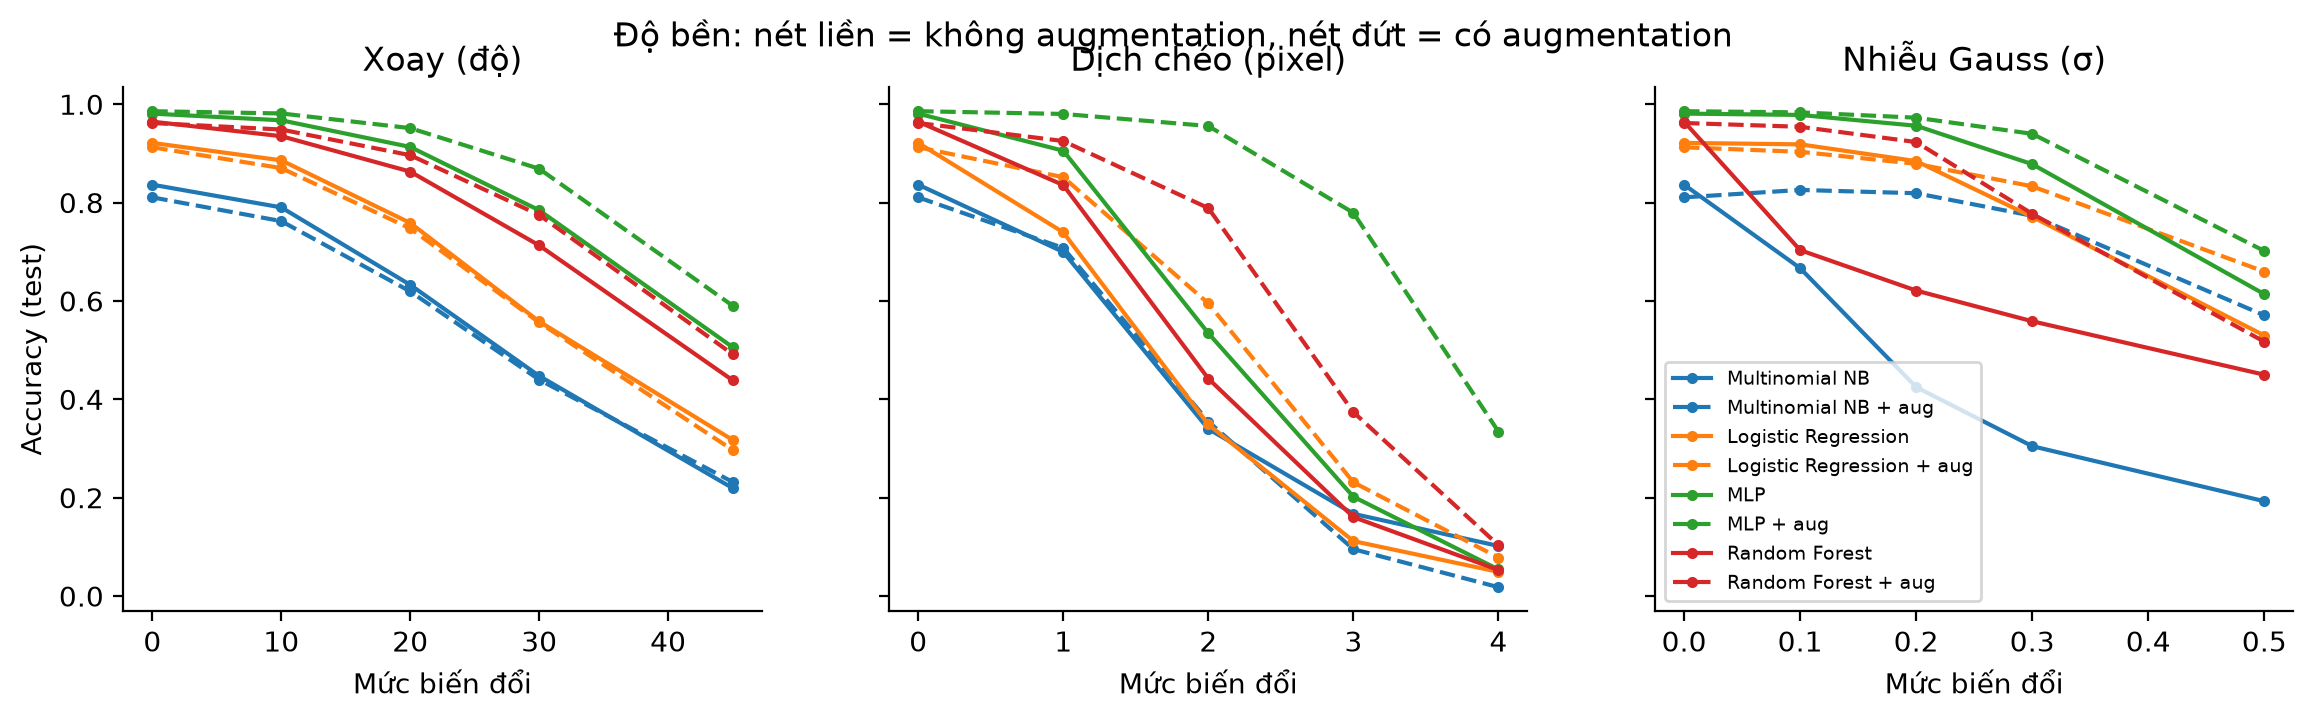
\includegraphics[width=0.9\textwidth]
        {figures/robustness_test.png}
        \caption{Sự thay đổi độ chính xác của các mô hình theo mức độ biến đổi ảnh}
        \label{fig:robustness}
    \end{minipage}
\end{figure}

\subsubsection{Nhận xét}

Kết quả cho thấy tăng cường dữ liệu cải thiện độ bền của một số
mô hình. Với phép xoay $30^\circ$, MLP có augmentation đạt
$86.88\%$, cao hơn mức $78.44\%$ của mô hình thông thường.
Khi dịch ảnh $3$ pixel, độ chính xác tăng từ $20.19\%$ lên
$77.91\%$. Random Forest cũng cải thiện ở cả hai phép biến đổi.

Ngược lại, Logistic Regression gần như không cải thiện khi xoay
ảnh, còn Multinomial Naive Bayes giảm độ chính xác sau augmentation.
Như vậy, hiệu quả của tăng cường dữ liệu phụ thuộc vào mô hình
và loại biến đổi, không phải lúc nào cũng mang lại kết quả tốt hơn.

Thí nghiệm này đánh giá độ bền trên ảnh MNIST bị biến đổi, chưa
đánh giá trực tiếp khả năng nhận dạng chữ số viết tay của người Việt.


\subsection{Giao diện demo vẽ và nhận diện chữ số}

\subsubsection{Mục đích}

Giao diện demo được xây dựng bằng thư viện Gradio, cho phép
người dùng vẽ trực tiếp chữ số viết tay từ 0 đến 9 và quan sát
kết quả nhận dạng. Hệ thống sử dụng bốn mô hình đã huấn luyện
gồm Multinomial Naive Bayes, Logistic Regression, MLP và
Random Forest. Các mô hình được lưu dưới dạng \texttt{.pkl}
trong thư mục \texttt{results/models/} và được tải khi khởi
chạy ứng dụng.

\subsubsection{Giao diện và chức năng}

Hình~\ref{fig:digit-demo-interface} minh họa giao diện demo
nhận diện chữ số viết tay. Các chức năng chính bao gồm:

\begin{itemize}
    \item \textbf{Vẽ chữ số:} Người dùng vẽ trực tiếp chữ số
    trên vùng vẽ của ứng dụng.

    \item \textbf{Tiền xử lý ảnh:} Ảnh đầu vào được chuyển
    sang mức xám, làm sạch và chuẩn hóa về kích thước
    $28\times28$ pixel.

    \item \textbf{Dự đoán:} Ảnh sau tiền xử lý được chuyển
    thành vector gồm 784 đặc trưng để đưa vào bốn mô hình.

    \item \textbf{Hiển thị kết quả:} Giao diện hiển thị các
    chữ số có xác suất dự đoán cao nhất của từng mô hình.

    \item \textbf{So sánh mô hình:} Hệ thống hiển thị thời gian
    dự đoán và thông báo khi các mô hình đồng thuận hoặc
    bất đồng về kết quả nhận dạng.
\end{itemize}

\begin{figure}[H]
    \centering
    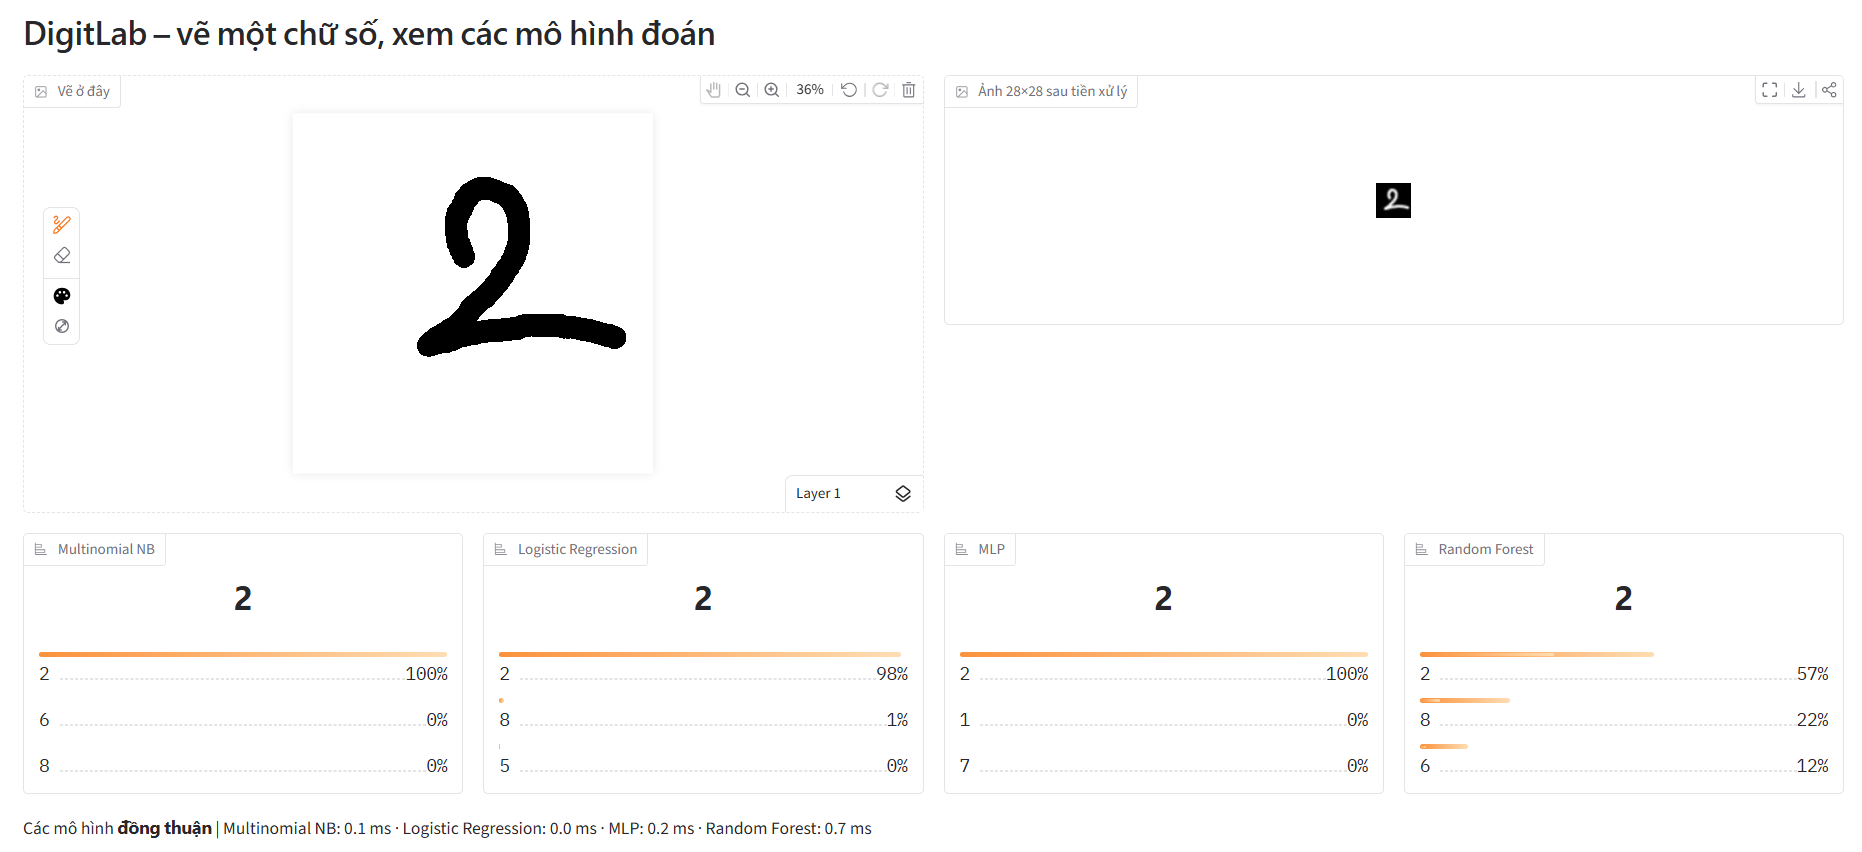
\includegraphics[
        width=0.82\textwidth,
        height=0.42\textheight,
        keepaspectratio
    ]{figures/digit_demo_interface.png}
    \caption{Giao diện demo nhận diện chữ số viết tay.}
    \label{fig:digit-demo-interface}
\end{figure}

\subsubsection{Quy trình nhận dạng}

Quy trình nhận dạng gồm hai phần: chuẩn bị mô hình đã huấn
luyện và xử lý ảnh đầu vào của người dùng. Các mô hình được
huấn luyện trong \texttt{main.ipynb}, lưu thành các tệp
\texttt{.pkl} và được tải trong \texttt{app.py}. Khi người
dùng vẽ chữ số, chương trình lần lượt thực hiện chuyển ảnh
sang mức xám, làm sạch, chuẩn hóa kích thước và chuyển ảnh
thành vector đặc trưng trước khi dự đoán.

Hình~\ref{fig:digit-demo-diagram} trình bày sơ đồ tổng quát
của quy trình này.

\begin{figure}[H]
    \centering
    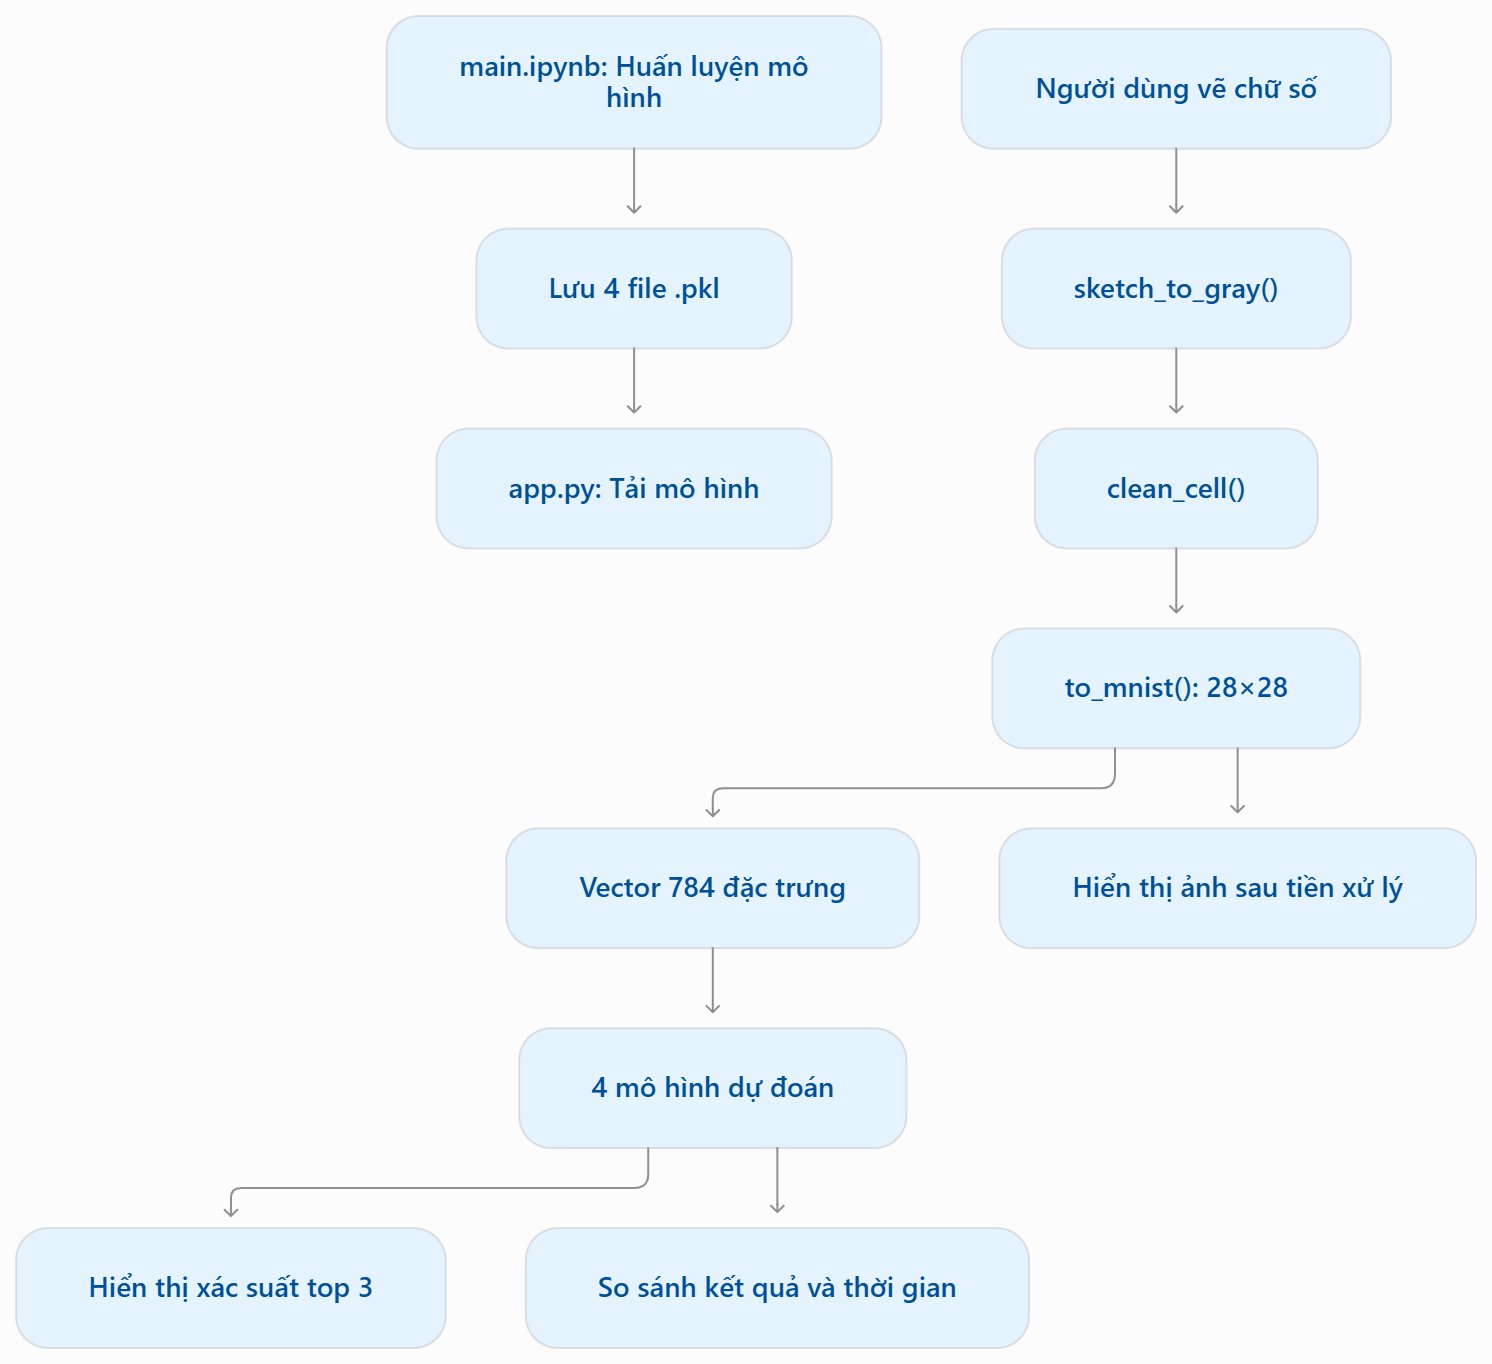
\includegraphics[
        width=0.88\textwidth,
        height=0.48\textheight,
        keepaspectratio
    ]{figures/digit_demo_diagram.png}
    \caption{Sơ đồ quy trình hoạt động của chương trình demo.}
    \label{fig:digit-demo-diagram}
\end{figure}

\subsubsection{Kiểm thử và minh họa kết quả}

Ngoài giao diện Gradio, quy trình nhận dạng còn được kiểm
thử trong \texttt{main.ipynb}. Chương trình tạo ảnh chữ số
minh họa, thực hiện tiền xử lý và đưa ảnh vào các mô hình
để quan sát kết quả dự đoán.

\begin{figure}[H]
    \centering
    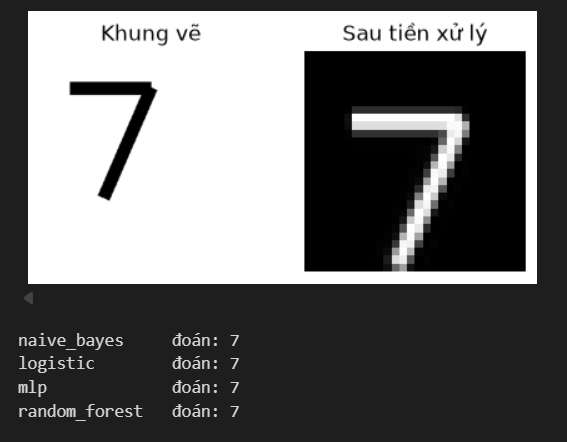
\includegraphics[
        width=0.78\textwidth,
        height=0.36\textheight,
        keepaspectratio
    ]{figures/digit_demo_inMain.png}
    \caption{Kiểm thử quy trình nhận dạng trong \texttt{main.ipynb}.}
    \label{fig:digit-demo-inmain}
\end{figure}

Để minh họa sự khác biệt giữa kết quả dự đoán của các mô
hình, Hình~\ref{fig:digit-demo-right} trình bày trường hợp
các mô hình đồng thuận, trong khi
Hình~\ref{fig:digit-demo-wrong} trình bày trường hợp các
mô hình đưa ra dự đoán khác nhau.

\begin{figure}[H]
    \centering
    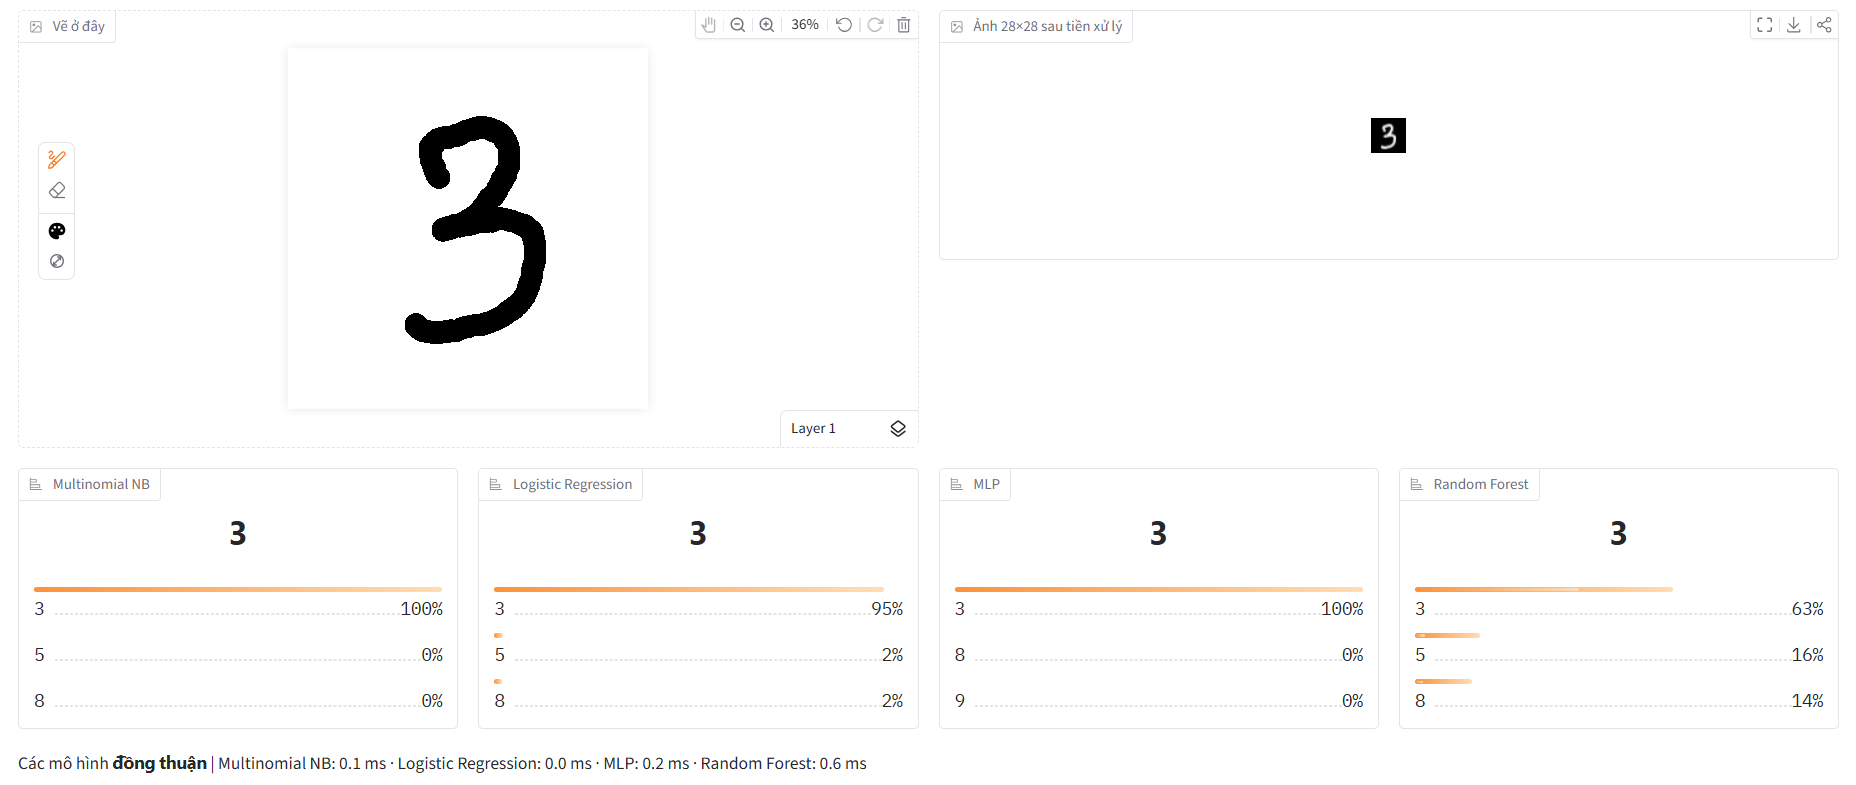
\includegraphics[
        width=0.78\textwidth,
        height=0.34\textheight,
        keepaspectratio
    ]{figures/digit_demo_right.png}
    \caption{Trường hợp các mô hình đồng thuận về kết quả dự đoán.}
    \label{fig:digit-demo-right}
\end{figure}

\begin{figure}[H]
    \centering
    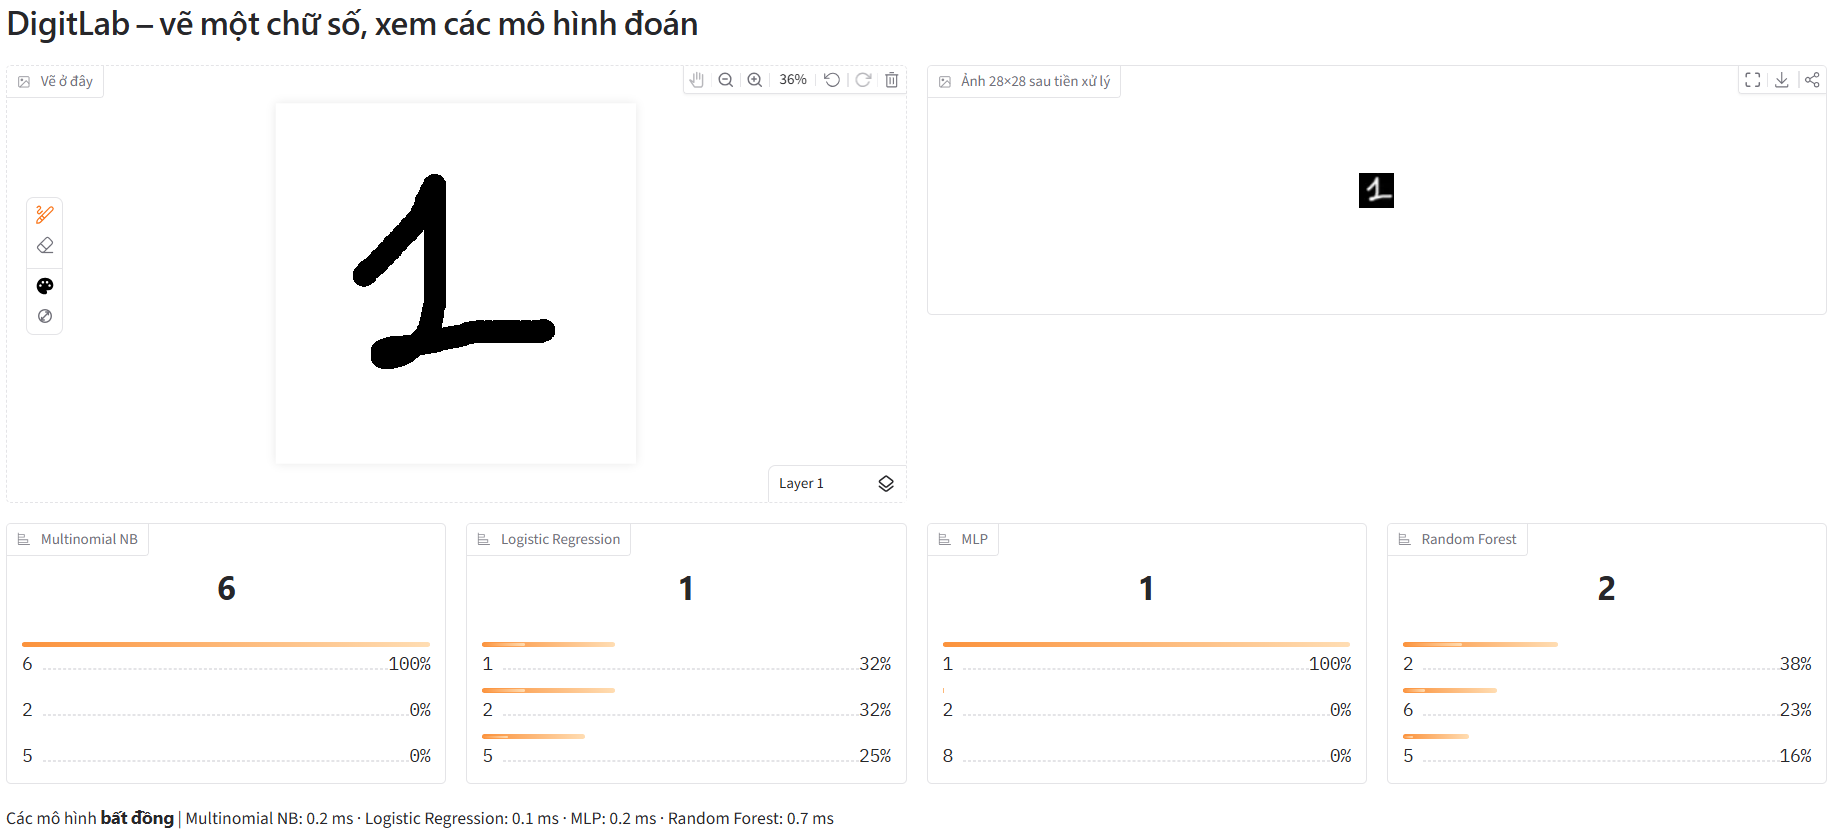
\includegraphics[
        width=0.78\textwidth,
        height=0.34\textheight,
        keepaspectratio
    ]{figures/digit_demo_wrong.png}
    \caption{Trường hợp các mô hình bất đồng về kết quả dự đoán.}
    \label{fig:digit-demo-wrong}
\end{figure}

\subsubsection{Đánh giá}

Giao diện demo giúp trực quan hóa quá trình nhận diện chữ số
viết tay, đồng thời hỗ trợ so sánh kết quả dự đoán và thời
gian suy luận của bốn mô hình. Tuy nhiên, việc các mô hình
đồng thuận không đồng nghĩa với dự đoán chính xác. Để xác
định trường hợp nhận dạng đúng hoặc sai, cần đối chiếu kết
quả dự đoán với nhãn thực tế của ảnh đầu vào. Các hình ảnh
minh họa chủ yếu phục vụ kiểm thử chức năng, không thay thế
cho việc đánh giá định lượng trên tập dữ liệu độc lập.
